\documentclass[a4paper,11pt]{article}
\usepackage{geometry}
 \geometry{
 a4paper,
 total={170mm,257mm},
 left=20mm,
 top=20mm,
 }

 \usepackage{multirow}
\usepackage{colortbl}
 \usepackage{hhline}

 \usepackage{lipsum}  %%% Lorem ipsum

\setlength{\headheight}{30.0pt}
\setlength{\footskip}{20pt}


\usepackage{hyperref}
\hypersetup{
    colorlinks=True,
    linkcolor={blue!20!black},
    filecolor=magenta,      
    urlcolor=cyan,
}



 \usepackage[export]{adjustbox}
\usepackage[english]{babel}
\usepackage[utf8]{inputenc}
\usepackage{fancyhdr}
\usepackage{multicol}

\pagestyle{fancy}
\fancyhf{}
\rhead{\textit{Pul074BEX004}}
\lhead{\textit{Amrit Prasad Phuyal}}
\rfoot{\thepage}


\usepackage{mathpazo} % Palatino font
\usepackage{graphicx}
\usepackage{float}

%%%% Anser environment use %%%% Anser environment use %%%% Anser environment use \input{./AnsENV.tex}
%% use \begin{A... {**** argument***}
\RequirePackage{scrextend}

\newenvironment{A}[1]{\textit{Answer:}{\begin{addmargin}[2em]{2em}{#1}\end{addmargin} 
  }}

% just leave some space   
%% use \begin{A... {**** argument***}
\RequirePackage{scrextend}

\newenvironment{A}[1]{\textit{Answer:}{\begin{addmargin}[2em]{2em}{#1}\end{addmargin} 
  }}

% just leave some space   
%% use \begin{A... {**** argument***}
\RequirePackage{scrextend}

\newenvironment{A}[1]{\textit{Answer:}{\begin{addmargin}[2em]{2em}{#1}\end{addmargin} 
  }}

% just leave some space    %% Answer environment 

%%% Question Environment%%%  use 
%%% Question Environment%%%  use 
%%% Question Environment%%%  use \input{./QueENV.tex}   to include
%% Use \begin{Q}....\end{Q}

\newcounter{QC}
\setcounter{QC}{1}
\newenvironment{Q}[1]{
    \section{Question -\arabic{QC}} \stepcounter{QC}{\large\textbf{#1}}
}

%%% Question Environment%%%

   to include
%% Use \begin{Q}....\end{Q}

\newcounter{QC}
\setcounter{QC}{1}
\newenvironment{Q}[1]{
    \section{Question -\arabic{QC}} \stepcounter{QC}{\large\textbf{#1}}
}

%%% Question Environment%%%

   to include
%% Use \begin{Q}....\end{Q}

\newcounter{QC}
\setcounter{QC}{1}
\newenvironment{Q}[1]{
    \section{Question -\arabic{QC}} \stepcounter{QC}{\large\textbf{#1}}
}

%%% Question Environment%%%

 %% Question Environment 
%%%%%% include  Titles.%%%% use \input{./CP}%%%
%%%use """"""""    \CP{}{}{}{}   """" %%%% and 4 argument to craete Title page 
%%%%%%%%%%%%%%%%%%%%%%%%%%%%%%%%%%%%%%%%%%%%%%%%%%%%%%%%%%%%%%%%%
%%%argument number
%% 1=major header ## Course name 
%% 2=minor4 heading ## lab/assignmet no
%% 3=Title  ## Assignment or Lab title
%% 4=submitted to::## input receiver Name"
%%%%%%%%%%%%%%%%%%%%%%%%%%%%%%%%%%%%%%%%%%%%%%%%%%%%%%%%%%%%%%%%%


\usepackage{mathpazo} % Palatino font
\usepackage{graphicx}
\usepackage{float}

%%% format and command for lab ans c and assembly

\newcommand{\HRule}{\rule{\linewidth}{0.4mm}} % Defines a new command for horizontal lines, change thickness here



%----------------------------------------------------------------------------------------
%	TITLE PAGE
%----------------------------------------------------------------------------------------


\newcommand{\CP}[4]{ \begin{titlepage} % Suppresses displaying the page number on the title page and the subsequent page counts as page 1
		%%%%  univerdity logo%%
		\begin{figure}[H]
			\centering
			
\includegraphics[scale=0.13]{tulogo.jpg}
		\end{figure}
		%%% end university logo

		\center % Centre everything on the page

		%------------------------------------------------
		%	Headings
		%------------------------------------------------

		\textsc{\huge Institute of Engineering \\ Central Campus,Pulchowk}\\[1.5cm] % Main heading such as the name of your university/college

		\textsc{\Large #1}\\[0.5cm] % Major heading such as course name

		\textsc{\large #2}\\[0.5cm] % Minor heading such as assignment no./ lab no.

		%------------------------------------------------
		%	Title
		%------------------------------------------------

		\HRule\\[0.4cm]

		{\Huge\bfseries #3}\\[0.4cm] % Title of your document

		\HRule\\[1.5cm]

		%------------------------------------------------
		%	Author(s)
		%------------------------------------------------
		\vfill\vfill
		\begin{minipage}{0.4\textwidth}
			\begin{flushleft}
				\large{
				\textbf{Submitted BY:}\\
				{\normalsize AMRIT PRASAD PHUYAL}\\ % NAME
				{\normalsize Roll: PULL074BEX004}} % Roll
			\end{flushleft}
		\end{minipage}
		~
		\begin{minipage}{0.4\textwidth}
			\begin{flushright}
				\large
				\textbf{Submitted To:}\\
				{ \normalsize{#4}\\ }% recepent's  Name 
				{\normalsize Department of Electronics and Computer Engineering}
			\end{flushright}
		\end{minipage}

		%------------------------------------------------
		%	Date
		%------------------------------------------------

		\vfill\vfill\vfill % Position the date 3/4 down the remaining page

		{\large\today} % Date, change the \today to a set date if you want to be precise

		\vfill % Push the date up 1/4 of the remaining page

	\end{titlepage}
} %%% cover page

%%% For CMD output %%%

%%%%%%%%% use  
%%% For CMD output %%%

%%%%%%%%% use  
%%% For CMD output %%%

%%%%%%%%% use  \include{CMD output.tex}
%%%%%%%%% use \CMD{###filename}{##Caption}
\usepackage{listings}

\usepackage{mdframed}
\usepackage{xcolor}
%\definecolor{codegreen}{rgb}{0,0.6,0}
%\definecolor{codegray}{rgb}{0.4,0.4,0.4}
%\definecolor{codepurple}{rgb}{0.58,0,0.82}
%\definecolor{blackcolour}{rgb}{0,0,0}


\definecolor{bluefront}{RGB}{10,214,255}
\definecolor{blueback}{RGB}{25,24,96}


\renewcommand{\lstlistlistingname}{List of CMD Outputs}
\renewcommand{\lstlistingname}{Output}


\lstdefinestyle{customa}{
    backgroundcolor=\color{blueback},
    %  keywordstyle=\color{magenta},
    %numberstyle=\tiny\color{codegray},
    %stringstyle=\color{codepurple},
    basicstyle=\ttfamily\scriptsize\color{bluefront},
    breakatwhitespace=false,
    breaklines=true,
    captionpos=b,
    %morekeywords={MOV,ADD,ADDC,ACALL,INC,DJNZ,AJMP,RET,END,ORG,RR,JNC,SUBB,JC,DEC},
    keepspaces=true,
    %numbers=left,
    %numbersep=5pt,
    showspaces=false,
    showstringspaces=false,
    showtabs=false,
    tabsize=4
}

\newcommand {\CMD}[2]{

    \begin{mdframed}[backgroundcolor=blueback,innerbottommargin=-2.3em,innertopmargin=-0.1em]
        \lstinputlisting[style=customa,caption={#2}]{#1}
    \end{mdframed}
}

%%% For CMD output %%%


%%%%%%%%% use \CMD{###filename}{##Caption}
\usepackage{listings}

\usepackage{mdframed}
\usepackage{xcolor}
%\definecolor{codegreen}{rgb}{0,0.6,0}
%\definecolor{codegray}{rgb}{0.4,0.4,0.4}
%\definecolor{codepurple}{rgb}{0.58,0,0.82}
%\definecolor{blackcolour}{rgb}{0,0,0}


\definecolor{bluefront}{RGB}{10,214,255}
\definecolor{blueback}{RGB}{25,24,96}


\renewcommand{\lstlistlistingname}{List of CMD Outputs}
\renewcommand{\lstlistingname}{Output}


\lstdefinestyle{customa}{
    backgroundcolor=\color{blueback},
    %  keywordstyle=\color{magenta},
    %numberstyle=\tiny\color{codegray},
    %stringstyle=\color{codepurple},
    basicstyle=\ttfamily\scriptsize\color{bluefront},
    breakatwhitespace=false,
    breaklines=true,
    captionpos=b,
    %morekeywords={MOV,ADD,ADDC,ACALL,INC,DJNZ,AJMP,RET,END,ORG,RR,JNC,SUBB,JC,DEC},
    keepspaces=true,
    %numbers=left,
    %numbersep=5pt,
    showspaces=false,
    showstringspaces=false,
    showtabs=false,
    tabsize=4
}

\newcommand {\CMD}[2]{

    \begin{mdframed}[backgroundcolor=blueback,innerbottommargin=-2.3em,innertopmargin=-0.1em]
        \lstinputlisting[style=customa,caption={#2}]{#1}
    \end{mdframed}
}

%%% For CMD output %%%


%%%%%%%%% use \CMD{###filename}{##Caption}
\usepackage{listings}

\usepackage{mdframed}
\usepackage{xcolor}
%\definecolor{codegreen}{rgb}{0,0.6,0}
%\definecolor{codegray}{rgb}{0.4,0.4,0.4}
%\definecolor{codepurple}{rgb}{0.58,0,0.82}
%\definecolor{blackcolour}{rgb}{0,0,0}


\definecolor{bluefront}{RGB}{10,214,255}
\definecolor{blueback}{RGB}{25,24,96}


\renewcommand{\lstlistlistingname}{List of CMD Outputs}
\renewcommand{\lstlistingname}{Output}


\lstdefinestyle{customa}{
    backgroundcolor=\color{blueback},
    %  keywordstyle=\color{magenta},
    %numberstyle=\tiny\color{codegray},
    %stringstyle=\color{codepurple},
    basicstyle=\ttfamily\scriptsize\color{bluefront},
    breakatwhitespace=false,
    breaklines=true,
    captionpos=b,
    %morekeywords={MOV,ADD,ADDC,ACALL,INC,DJNZ,AJMP,RET,END,ORG,RR,JNC,SUBB,JC,DEC},
    keepspaces=true,
    %numbers=left,
    %numbersep=5pt,
    showspaces=false,
    showstringspaces=false,
    showtabs=false,
    tabsize=4
}

\newcommand {\CMD}[2]{

    \begin{mdframed}[backgroundcolor=blueback,innerbottommargin=-2.3em,innertopmargin=-0.1em]
        \lstinputlisting[style=customa,caption={#2}]{#1}
    \end{mdframed}
}

%%% For CMD output %%%

 %%% Cmd OUTPUT blue background


\begin{document}


%%%%  COver page 
\CP{Computer Network}{Lab \#8}{VLAN Configuration, Forwarding Packets within VLAN and Routing
    packets between VLANs}
{SHARAD KUMAR GHIMIRE}
%%%%%%%%%%%%%%%%%%%%

\pagenumbering{gobble}
\renewcommand{\contentsname}{Table of Contents}
\tableofcontents

%\pagebreak
%\listoffigures
% \pagebreak
% \listoftables
\pagebreak
\lstlistoflistings
\pagebreak
\listoffigures
\pagebreak
\pagenumbering{arabic}

\section{Title} {\large VLAN Configuration, Forwarding Packets within VLAN and Routing
  packets between VLANs}
%%%%%%%%%%%%%%%%%%%%%%%%%%%%
\section{Objective}
\begin{itemize}
    \item To be familiar with VLAN and its use
    \item To create VLANs and deliver packets between computers that are within the same VLAN
    \item To route packets between computers at different VLANs
\end{itemize}
%%%%%%%%%%%%%%%%%%%%%
\section{Requirement}
\begin{itemize}
    \item Network simulation tool: Packet Tracer
\end{itemize}
%%%%%%%%%%%%%%%%%%%

\section{Procedure}

With the help of Cisco Packet Tracer we simulated VLANs. we also explored the packet forwarding within VLAN and Routing them between VLANs.

\pagebreak
\section{Exercises:}

%%%%%%%%%%%%%%%%%%%%%%%%%11111111111111111111111
%%%%%%%%%%%%%%%%%%%%%%%%%%%%
\begin{Q}
    {
        What is VLAN? Explain its importance in networking.
    }
\end{Q}

\begin{A}
    {
        VLAN (Virtual LAN) divides broadcast domain in devices like Switch. In other terms its a technique to create a sub network of devices situated physically on different LANs.

        The needs of VLAN in networking are as follows :
        \begin{itemize}
            \item Improve security as it limits access  to devices and users.
            \item Improved manageability as it has feature to group devices and user with similar requirement or function
            \item Reduces overall IT cost as it eliminated the need of actual physical hardware and wires.
        \end{itemize}
    }
\end{A}
%%%%%%%%%%%%%%%%%%%%%%%%%%%%%%%%%%%%%%%%%%%%%%%%%%%%%%%%%%%%%%%%%%%

%%%%%%%%%%%%%%%%%%%%%%%%%%%%22222222222222222222222222222
\begin{Q}
    {
        How VLAN can be configured? Explain each step in detail.
    }
\end{Q}


VLAN can be Configures in two steps :

\begin{itemize}
    \item \textbf{Creating VLANs}
          \begin{verbatim}
Switch> enable
Switch# configure terminal
Switch(config)# vlan vlan_ID
Switch(config-vlan)# name Vlan_2
Switch(config-vlan)# end
Switch#  \end{verbatim}
    \item  \textbf{Assigning an Interface to Particular Vlan}
          \begin{verbatim}
 Switch> enable 
 Switch# configure terminal
 Switch(config)#interface FastEthernet0/11
 Switch(config-if)#switchport access vlan 2
 Switch(config-if)#end
 Switch#  \end{verbatim}
\end{itemize}

%%%%%%%%%%%%%%%%%%%%%%%%%%%%%%%%%%%%%%%%%%%%%%%%%%%%%%%%%%%%%%%%%%%

%%%%%%%%%%%%%%%%%%%%%%%%%%%%33333333333333333333333333333333333
\begin{Q}
    {
        How packets can be forwarded between computers within same VLAN but connected at
        different switches? Explain.
    }
\end{Q}

\begin{A}
    {
        Concept Trunk can be implemented if two devices on same VLAN but different Switches has to communicate. In trunk mode Trunking protocols include VLAN information in each frame transmitting through it.The receiving end forwards the packets to destination after deframing the VLAN info. This has been implemented and tested starting from \textbf{Activity B.1} .\\

        Another Simpler method is to simply add extra interface corresponding to particular VLAN .This has been implemented and tested in \textbf{Activity A.7}
    }
\end{A}
%%%%%%%%%%%%%%%%%%%%%%%%%%%%%%%%%%%%%%%%%%%%%%%%%%%%%%%%%%%%%%%%%%%

%%%%%%%%%%%%%%%%%%%%%%%%%%%%4444444444444444444444444444444444444
\begin{Q}
    {
        How packets can be routed between computers at different VLANs? Explain.
    }
\end{Q}

\begin{A}
    {
        An Router can provide a viable solution to our problem as its primary task is to route the packets between different network or sub network like VLAN.Router can be connected in two ways . One is to separately connects interfaces connecting belonging to VLANs and other is to use trunk and sub interface technique to achieve similar functionality using single interface. These are Implemented in \textbf{Activity C and D}\\

        Another Simpler method is to introduce $3^{rd}$ Switch that simply connects the interfaces belonging to different VLAN.For this to work they must belong to same subnet.This has been implemented and tested in \textbf{Activity B.6}
    }
\end{A}
%%%%%%%%%%%%%%%%%%%%%%%%%%%%%%%%%%%%%%%%%%%%%%%%%%%%%%%%%%%%%%%%%%%

%%%%%%%%%%%%%%%%%%%%%%%%%%%%555555555555555555555555555555555555
\begin{Q}
    {
        Note down the results of each and step of above exercise also explain with reason.
    }
\end{Q}

%
%
%
%

%%%%%%%%%%%%%%%%%%%%%%AAAAAAAAAAAAAAAAAAAAAA
%%%%%%%%%%%%%%%%%%%%%%AAAAAAAAAAAAAAAAAAAAAA
%%%%%%%%%%%%%%%%%%%%%%AAAAAAAAAAAAAAAAAAAAAA
%%%%%%%%%%%%%%%%%%%%%%AAAAAAAAAAAAAAAAAAAAAA
%%%%%%%%%%%%%%%%%%%%%%AAAAAAAAAAAAAAAAAAAAAA
%
%

%
%
\addtocontents{lol}{\protect\subsection*{\HRule \\ Activities A\\ \HRule}}

\addtocontents{lof}{\protect\subsection*{\HRule \\ Activities A\\ \HRule}}

\subsubsection{Activities A}

{\bfseries \textit{A. Create the network topology as shown in figure 1 below and perform the following activities:}}




\begin{enumerate}
    %%%%%%%%%%%%%%%%%%%%%%AAAAAAAAAAAAAAAAAAAAAA11111111111111111111111111
    \item\textbf{ Connect the computers and switches as followings:
              \begin{itemize}
                  \item  Connect PC0 and PC1 to interfaces FastEthernet 0/1 and FastEthernet 0/11 of switch0
                        respectively
                  \item Connect PC2 and PC3 to interfaces FastEthernet 0/1 and FastEthernet 0/11 of switch1
                        respectively
                  \item  Connect interfaces FastEthernet 0/10 of Switch0 with FastEthernet 0/10 of Switch1
                  \item Assign IP address and subnet mask of computers as:
                        \begin{itemize}
                            \item  PC0: 200.1.1.2/24
                            \item  PC1: 200.1.1.66/24
                            \item  PC2: 200.1.1.3/24
                            \item  PC3: 200.1.1.67/24
                        \end{itemize}
              \end{itemize} }

          \begin{figure}[H]
              \centering
              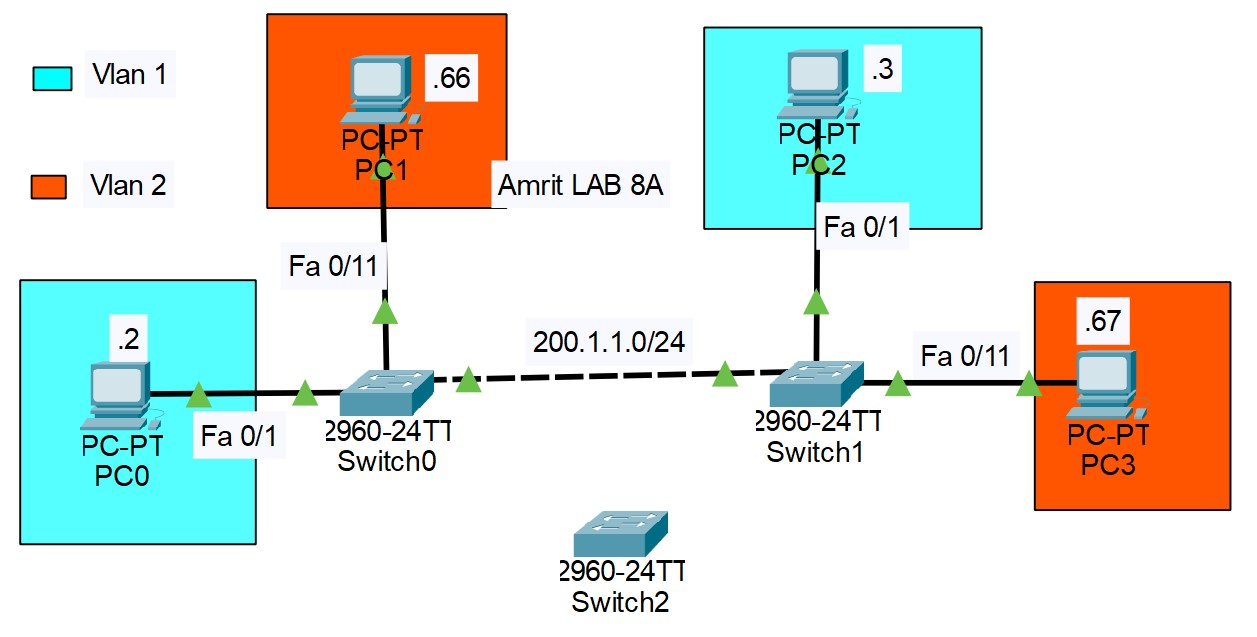
\includegraphics[scale=0.68,cframe=blue 0.5pt 3pt]{./FIG/Lab8A.jpg}
              \caption{Network topology Lab 8A}
          \end{figure}


          %%%%%%%%%%%%%%%%%%%%%%AAAAAAAAAAAAAAAAAAAAAA222222222222222222222222
    \item\textbf{ Observe the result by testing the connectivity between each computers}



          \addtocontents{lol}{\protect\subsubsection*{A.2 : Testing connectivity before configuring VLAN}}

          \CMD{./CODES/AP0-1.txt}{Ping from PC0 to PC1}

          \CMD{./CODES/AP0-2.txt}{Ping from PC0 to PC2}

          \CMD{./CODES/AP0-3.txt}{Ping from PC0 to PC3}

          \CMD{./CODES/AP1-2.txt}{Ping from PC1 to PC2}

          \CMD{./CODES/AP1-3.txt}{Ping from PC1 to PC3}

          \CMD{./CODES/AP2-3.txt}{Ping from PC2 to PC3}


          Since all PCs falls under same VLAN \textit{i.e.} 1 and all assigned IPs belongs to same subnet all PCs can communicate with each other.

          %%%%%%%%%%%%%%%%%%%%%%AAAAAAAAAAAAAAAAAAAAAA333333333333333333333333
    \item\textbf{ Create the VLAN 2 in both switches i.e. Switch0 and Switch1}

          \addtocontents{lol}{\protect\subsubsection*{A.3 : Creating VLAN}}


          \CMD{./CODES/A_CVS0.txt}{Create VLAN in switch 0}

          \CMD{./CODES/A_CVS1.txt}{Create VLAN in switch 1}

          %%%%%%%%%%%%%%%%%%%%%%AAAAAAAAAAAAAAAAAAAAAA444444444444444444444444444
    \item\textbf{ Assign interfaces FastEthernet 0/11, 0/12, 0/13, 0/14 of both switches to VLAN 2}

          \addtocontents{lol}{\protect\subsubsection*{A.4 : Assigning Interfaces to VLAN}}

          \CMD{./CODES/A_IS1.txt}{Assigning Interfaces to VLAN in Switch 1}
          \CMD{./CODES/A_IS0.txt}{Assigning Interfaces to VLAN in Switch 0}

          %%%%%%%%%%%%%%%%%%%%%%AAAAAAAAAAAAAAAAAAAAAA5555555555555555555555555555555
    \item\textbf{ Observe the result by testing the connectivity between each computers}


          \addtocontents{lol}{\protect\subsubsection*{A.5 : Testing connectivity after configuring VLAN}}

          \CMD{./CODES/APV0-1.txt}{Ping from PC0 to PC1}

          \CMD{./CODES/APV0-2.txt}{Ping from PC0 to PC2}

          \CMD{./CODES/APV0-3.txt}{Ping from PC0 to PC3}

          \CMD{./CODES/APV1-2.txt}{Ping from PC1 to PC2}

          \CMD{./CODES/APV1-3.txt}{Ping from PC1 to PC3}

          \CMD{./CODES/APV2-3.txt}{Ping from PC2 to PC3}

          Though the assigned IPs belongs to same subnet the  PC0 and PC2 falls under same VLAN \textit{i.e.} 1 and (PC1 and PC3) falls under another  VLAN \textit{i.e.} 2. PCs of different VlAN cant communicate with each other as only one interface corresponding to VlAN 1 is connected between switch.


          %%%%%%%%%%%%%%%%%%%%%%AAAAAAAAAAAAAAAAAAAAAA666666666666666666666666
    \item\textbf{ Does the ping from PC1 to PC3 succeed? State reason.}

          Ping failed as shown in above Output. Though, they both belongs to same VLAN and same subnet only interface for VLAN 1 is connected between switch 0 and switch 1 ping failed.


          %%%%%%%%%%%%%%%%%%%%%%AAAAAAAAAAAAAAAAAAAAAA777777777777777777777777777777777
    \item\textbf{ Connect interface FastEthernet 0/12 of Switch0 with FastEthernet 0/12 of Switch1}


          \begin{figure}[H]
              \centering
              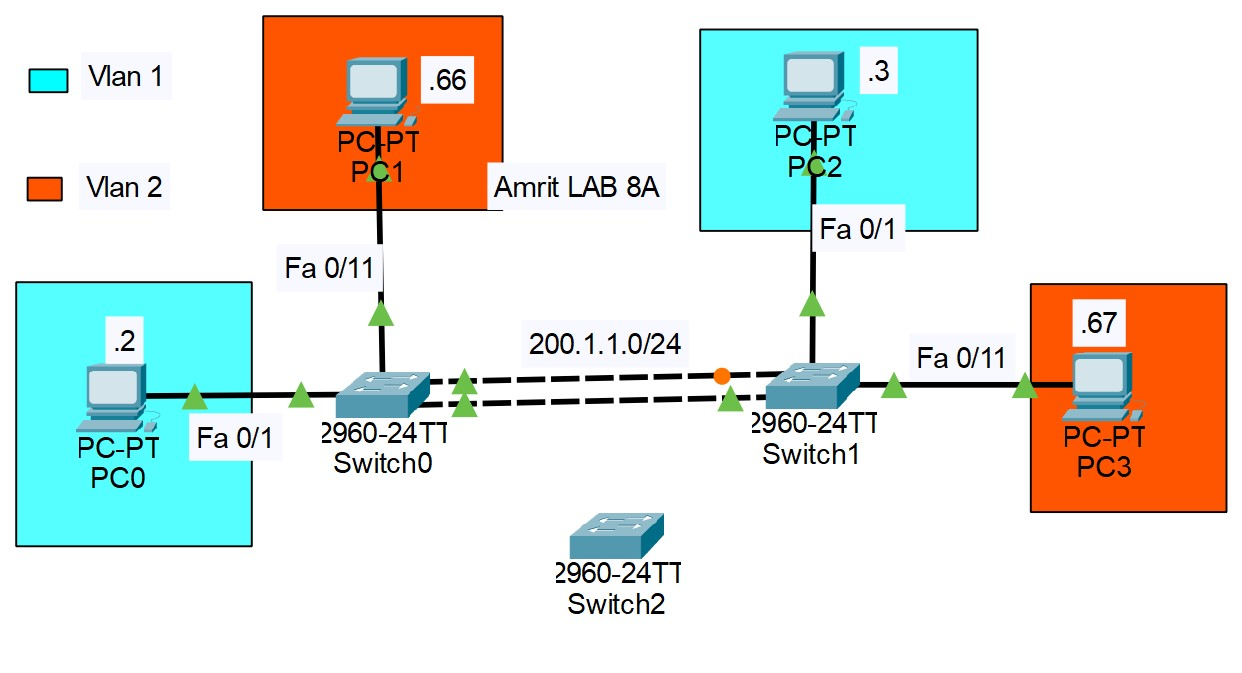
\includegraphics[scale=0.68,cframe=blue 0.5pt 3pt]{./FIG/Lab8A7.jpg}
              \caption{Network topology Lab 8A after interconnecting additional interface between Switch0  and Switch 1 }
          \end{figure}




          %%%%%%%%%%%%%%%%%%%%%%AAAAAAAAAAAAAAAAAAAAAA888888888888888888888888888888888888
    \item\textbf{ Observe the result by testing the connectivity between each computers}


          \addtocontents{lol}{\protect\subsubsection*{A.8 : Testing connectivity after interconnecting extra interface Between Switches}}

          \CMD{./CODES/APE0-1.txt}{Ping from PC0 to PC1}

          \CMD{./CODES/APE0-2.txt}{Ping from PC0 to PC2}

          \CMD{./CODES/APE0-3.txt}{Ping from PC0 to PC3}

          \CMD{./CODES/APE1-2.txt}{Ping from PC1 to PC2}

          \CMD{./CODES/APE1-3.txt}{Ping from PC1 to PC3}

          \CMD{./CODES/APE2-3.txt}{Ping from PC2 to PC3}



          %%%%%%%%%%%%%%%%%%%%%%AAAAAAAAAAAAAAAAAAAAAA999999999999999999999999999999999
    \item\textbf{ Does the ping from PC1 to PC3 succeed? State reason.}

          Yes ping from PC1 to PC3 succeed. Here we introduced additional interface between the switches FastEthernet 0/12 belonging to VLAN 2 the communication between the PCs belonging to same VLAN but connected to different switches is possible.


          %%%%%%%%%%%%%%%%%%%%%%AAAAAAAAAAAAAAAAAAAAAA10 10 10 10 10 10 10 10
    \item\textbf{ Does the ping from PC0 to PC1 succeed? State reason.}

          No, the Ping failed simply because they belong to different VLAN.



          %%%%%%%%%%%%%%%%%%%%%%AAAAAAAAAAAAAAAAAAAAAA11 11 11 11 11 11 11 11 11 11 11
    \item\textbf{ Now connect interface FastEthernet 0/9 of Switch1 with FastEthernet 0/9 of Switch2 and
              FastEthernet 0/13 of Switch1 with FastEthernet 0/13 of Switch2}

          \begin{figure}[H]
              \centering
              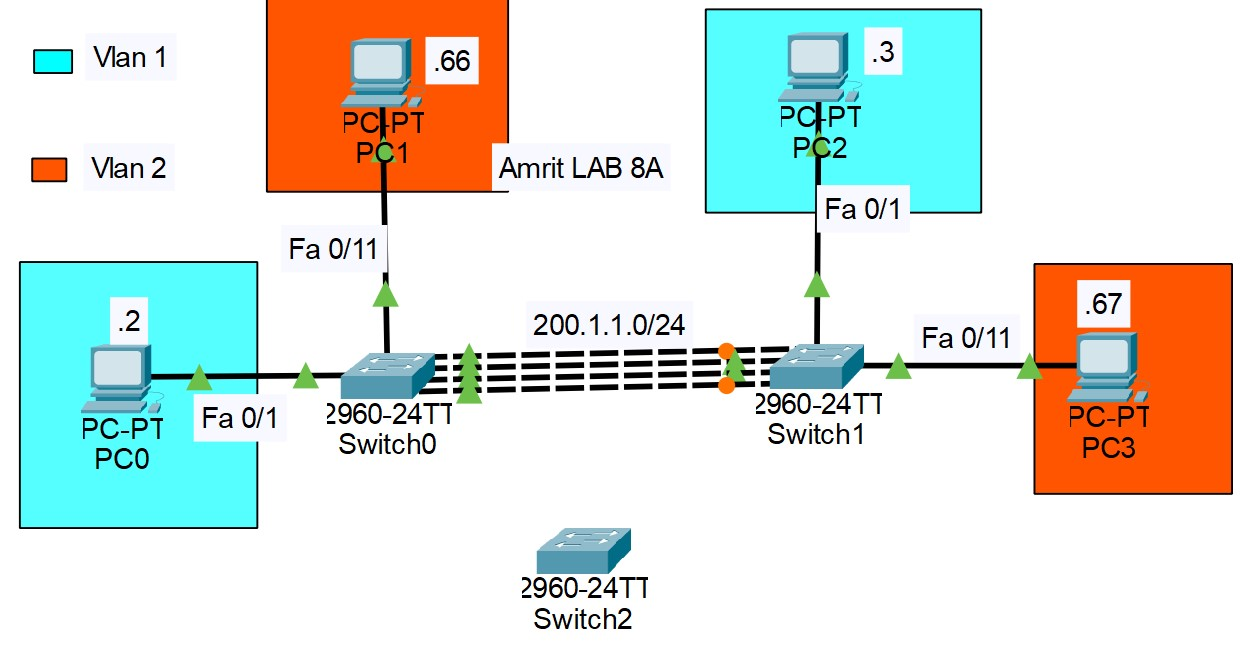
\includegraphics[scale=0.66,cframe=blue 0.5pt 3pt]{./FIG/Lab8A11.jpg}
              \caption{Network topology Lab 8A after interconnecting 2 additional interface between Switch0  and Switch 1 }
          \end{figure}




          %%%%%%%%%%%%%%%%%%%%%%AAAAAAAAAAAAAAAAAAAAAA12 12 12 12 12 12 12 12 
    \item\textbf{ Observe the result by testing the connectivity between each computers}


          \addtocontents{lol}{\protect\subsubsection*{A.12 : Testing connectivity after interconnecting 2 additional interface Between Switches 1 and 2}}

          %%%%%%%%%%%%%%%%%%%%Copied from A.8 don't make changes, if needed create new


          \CMD{./CODES/AP0-1.txt}{Ping from PC0 to PC1}

          \CMD{./CODES/AP0-2.txt}{Ping from PC0 to PC2}

          \CMD{./CODES/AP0-3.txt}{Ping from PC0 to PC3}

          \CMD{./CODES/AP1-2.txt}{Ping from PC1 to PC2}

          \CMD{./CODES/AP1-3.txt}{Ping from PC1 to PC3}

          \CMD{./CODES/AP2-3.txt}{Ping from PC2 to PC3}

          Ping is successful between all PCs when third switch is used to interconnect VLAN 1 and VLAN 2. The third switch simply acts as switch to connect two different LAN. Additionally, all assigned IPs falls under same subnet.

          %%%%%%%%%%%%%%%%%%%%%%AAAAAAAAAAAAAAAAAAAAAA13 13 13 13 13 13 13 13 13 13
    \item\textbf{ Does the ping from PC0 to PC1 succeed? State reason.}
          As shown in above outputs the ping success. Though PC0 and PC1 belongs to different VLAN the new switch connects these VLAN as normal LAN and enable communication between them.

\end{enumerate}


\pagebreak
%
%
%
%

%%%%%%%%%%%%%%%%%%%%%%BBBBBBBBBBBBBBBBBBBBBBBBBBBBBBBBB
%%%%%%%%%%%%%%%%%%%%%%BBBBBBBBBBBBBBBBBBBBBBBBBBBBBBBBB
%%%%%%%%%%%%%%%%%%%%%%BBBBBBBBBBBBBBBBBBBBBBBBBBBBBBBBB
%%%%%%%%%%%%%%%%%%%%%BBBBBBBBBBBBBBBBBBBBBBBBBBBBBBBBB
%%%%%%%%%%%%%%%%%%%%%%BBBBBBBBBBBBBBBBBBBBBBBBBBBBBBBBB

%
%
%


\addtocontents{lol}{\protect\subsection*{\HRule \\ Activities B\\ \HRule}}

\addtocontents{lof}{\protect\subsection*{\HRule \\ Activities B\\ \HRule}}

\subsubsection{Activities B}

{\bfseries \textit{B. From the above network topology remove all links between switches, and perform the
        followings:}}



\begin{enumerate}

    %%%%%%%%%%%%%%%%%%%%%%BBBBBBBBBBBBBBBBBBBBBBBBBBBBBBBBB11111111111111111111111111
    \item\textbf{ Configure interfaces FastEthernet0/20 of both switches Switch0 and Switch1 as Trunk
              port and establish connection between two switches using these ports}

          \addtocontents{lol}{\protect\subsubsection*{B.1 : Configuring Trunk port in both switches }}


          \begin{figure}[H]
              \centering
              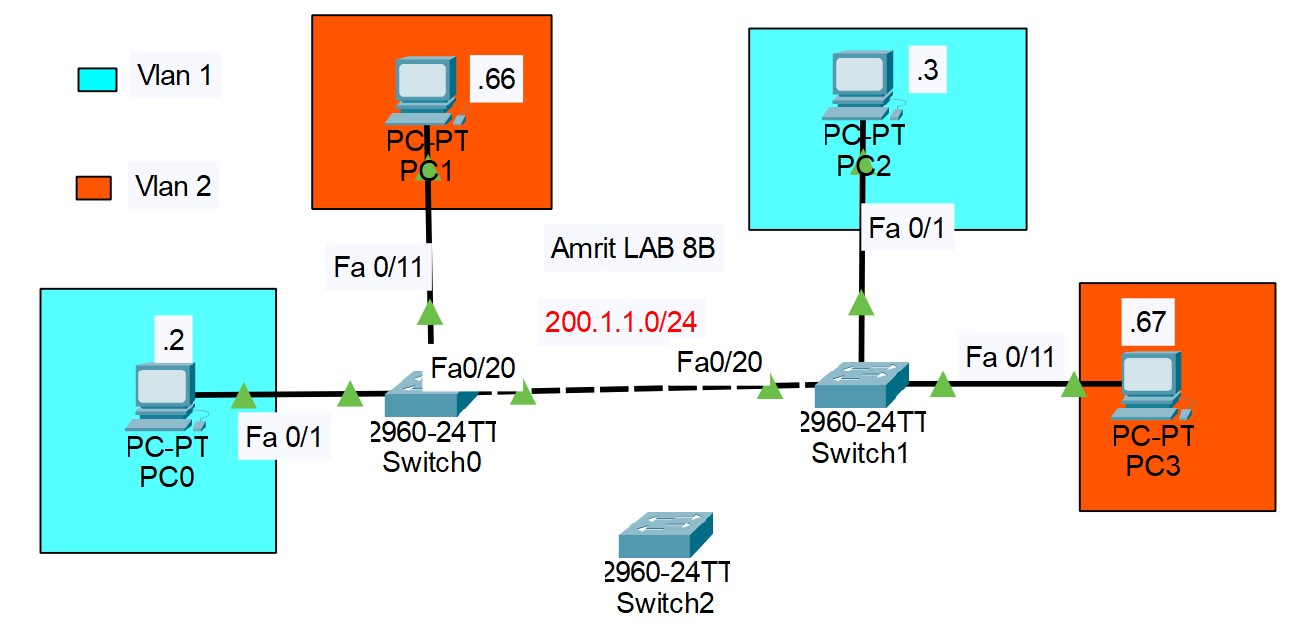
\includegraphics[scale=0.67,cframe=blue 0.5pt 3pt]{./FIG/Lab8B1.jpg}
              \caption{Network topology Lab 8B after configuring Trunk port }
          \end{figure}


          Here we reduced the number of interface needed to connect both VLAN in Both switches with the help of trunk protocol.

          \CMD{./CODES/B_CI0.txt}{Configure Fa 0/20 for trunk in switch 0}

          \CMD{./CODES/B_CI1.txt}{Configure Fa 0/20 for trunk in switch 1}



          %%%%%%%%%%%%%%%%%%%%%%BBBBBBBBBBBBBBBBBBBBBBBBBBBBBBBBB222222222222222222222
    \item\textbf{  Observe the result by testing the connectivity between each computers}

          \addtocontents{lol}{\protect\subsubsection*{B.2 : Testing connectivity after Configuring Trunk for Fa 0/20}}

          \CMD{./CODES/BPT0-1.txt}{Ping from PC0 to PC1}

          \CMD{./CODES/BPT0-2.txt}{Ping from PC0 to PC2}

          \CMD{./CODES/BPT0-3.txt}{Ping from PC0 to PC3}

          \CMD{./CODES/BPT1-2.txt}{Ping from PC1 to PC2}

          \CMD{./CODES/BPT1-3.txt}{Ping from PC1 to PC3}

          \CMD{./CODES/BPT2-3.txt}{Ping from PC2 to PC3}

          In this activity we only reduced the number of Interface connected between Switch 0 and Switch 1 and additionally disconnect the switch 1 and switch 2 which make the communication between VLAN 1 and VLAN 2 impossible.

          %%%%%%%%%%%%%%%%%%%%%%BBBBBBBBBBBBBBBBBBBBBBBBBBBBBBBBB33333333333333333333333333333
    \item\textbf{  Does the ping from PC0 to PC1 succeed? State reason}
          PC0 and PC1 falls under same subnet but belongs to different VLAN and here we disconnected the interfaces with switch 2 that was previously used to make connection between VLANs.


          %%%%%%%%%%%%%%%%%%%%%%BBBBBBBBBBBBBBBBBBBBBBBBBBBBBBBBB444444444444444444444444444444
    \item\textbf{  Does the ping from PC0 to PC2 succeed? State reason}
          Yes the ping between PC0 and PC2 succeed as they belong to same VLAN, same Subnet and there is trunk to connect two switches.

          %%%%%%%%%%%%%%%%%%%%%%BBBBBBBBBBBBBBBBBBBBBBBBBBBBBBBBB555555555555555555555555555555
    \item\textbf{  Does the ping from PC1 to PC3 succeed? State reason}

          Yes the ping between PC1 and PC3 succeed as they belong to same VLAN, same Subnet and there is trunk to connect two switches.

          %%%%%%%%%%%%%%%%%%%%%%BBBBBBBBBBBBBBBBBBBBBBBBBBBBBBBBB66666666666666666666666666666666
    \item\textbf{  Interconnect two VLANs using another switch as: Connect interface FastEthernet0/9 of
              Switch1 with FastEthernet0/9 of Switch2 and FastEthernet0/13 of Switch1 with
              FastEthernet0/13 of Switch2 and repeat from ii to v}


          \begin{figure}[H]
              \centering
              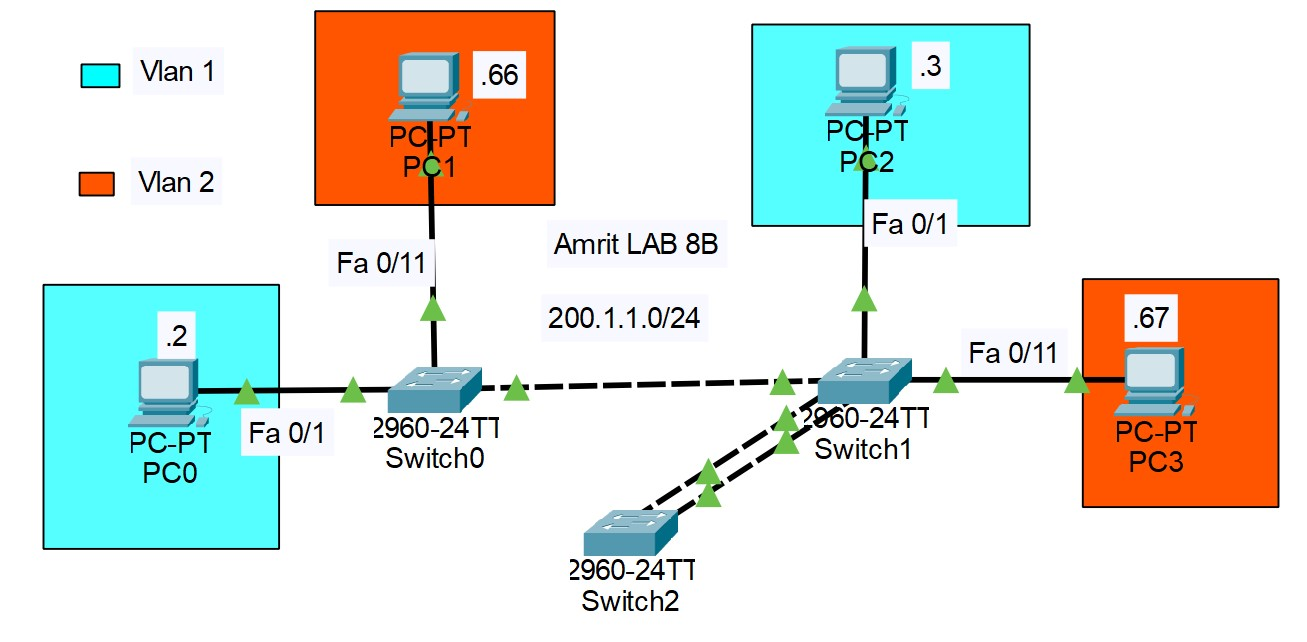
\includegraphics[scale=0.65,cframe=blue 0.5pt 3pt]{./FIG/Lab8B7.jpg}
              \caption{Network topology Lab 8B after connecting Switch 2 }
          \end{figure}


          \begin{enumerate}
              \item\textbf{Observe the result by testing the connectivity between each computers}

                    \addtocontents{lol}{\protect\subsubsection*{B.6 : Testing connectivity  after connecting Switch 2}}

                    \CMD{./CODES/BPS0-1.txt}{Ping from PC0 to PC1}

                    \CMD{./CODES/BPS0-2.txt}{Ping from PC0 to PC2}

                    \CMD{./CODES/BPS0-3.txt}{Ping from PC0 to PC3}

                    \CMD{./CODES/BPS1-2.txt}{Ping from PC1 to PC2}

                    \CMD{./CODES/BPS1-3.txt}{Ping from PC1 to PC3}

                    \CMD{./CODES/BPS2-3.txt}{Ping from PC2 to PC3}

                    In this activity we only reduced the number of Interface connected between Switch 0 and Switch 1 with the help of Trunk mode and additionally connect the switch 1 and switch 2 which make the communication between VLAN 1 and VLAN 2 possible.

              \item\textbf{  Does the ping from PC0 to PC1 succeed? State reason}
                    Ping is successful as PC0 and PC1 falls under same subnet but belongs to different VLAN and here we connected the interfaces with switch 2 that is used to make connection between VLANs.


                    %%%%%%%%%%%%%%%%%%%%%%BBBBBBBBBBBBBBBBBBBBBBBBBBBBBBBBB444444444444444444444444444444
              \item\textbf{  Does the ping from PC0 to PC2 succeed? State reason}
                    Yes the ping between PC0 and PC2 succeed as they belong to same VLAN, same Subnet and there is trunk to connect two switches.

                    %%%%%%%%%%%%%%%%%%%%%%BBBBBBBBBBBBBBBBBBBBBBBBBBBBBBBBB555555555555555555555555555555
              \item\textbf{  Does the ping from PC1 to PC3 succeed? State reason}

                    Yes the ping between PC1 and PC3 succeed as they belong to same VLAN, same Subnet and there is trunk to connect two switches.

          \end{enumerate}



          %%%%%%%%%%%%%%%%%%%%%%BBBBBBBBBBBBBBBBBBBBBBBBBBBBBBBBB7777777777777777777777777777
    \item\textbf{  Compare the current configuration with above}

          Here we have Introduced the Switch 2 that connect VLAN 1 and VLAN 2 and make connection possible between them.

\end{enumerate}

\pagebreak
%%%%%%%%%%%%%%%%%%%%%%%%%%%%%%%%%%%%%%%%%%%%%%%%%%%%%%%%%%%%%%%%%%%
%%%%%%%

%

%

%

%
%%%%%%%%%%%%%%%%CCCCCCCCCCCCCCCCCCCCC
%%%%%%%%%%%%%%%%CCCCCCCCCCCCCCCCCCCCC
%%%%%%%%%%%%%%%%CCCCCCCCCCCCCCCCCCCCC
%%%%%%%%%%%%%%%%CCCCCCCCCCCCCCCCCCCCC
%%%%%%%%%%%%%%%%CCCCCCCCCCCCCCCCCCCCC
%

%

%

%

\addtocontents{lol}{\protect\subsection*{\HRule \\ Activities C\\ \HRule}}

\addtocontents{lof}{\protect\subsection*{\HRule \\ Activities C\\ \HRule}}

\subsubsection{Activities C}

{\bfseries \textit{C. From the above condition of question no. 2, change the subnet mask to 255.255.255.192, and
        perform the followings:}}


\begin{figure}[H]
    \centering
    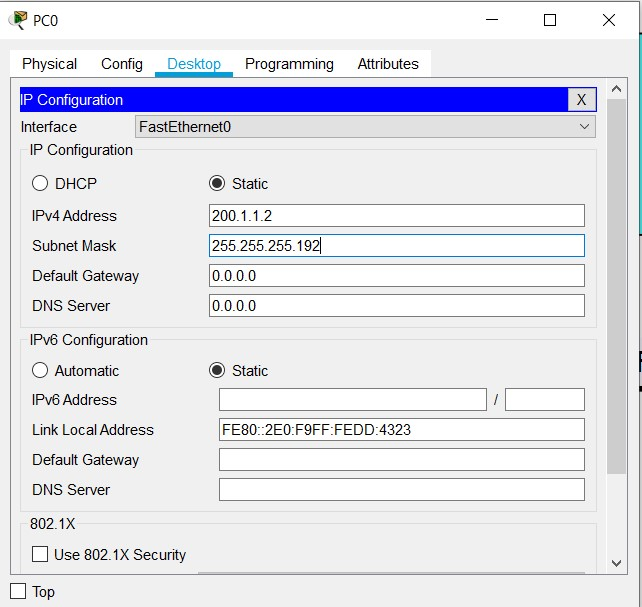
\includegraphics[scale=0.82,cframe=blue 0.5pt 3pt]{./FIG/C_SP0.jpg}
    \caption{Changing Subnet for Lab 8c in PC0 to 255.255.255.192 or /26 }
\end{figure}


\begin{figure}[H]
    \centering
    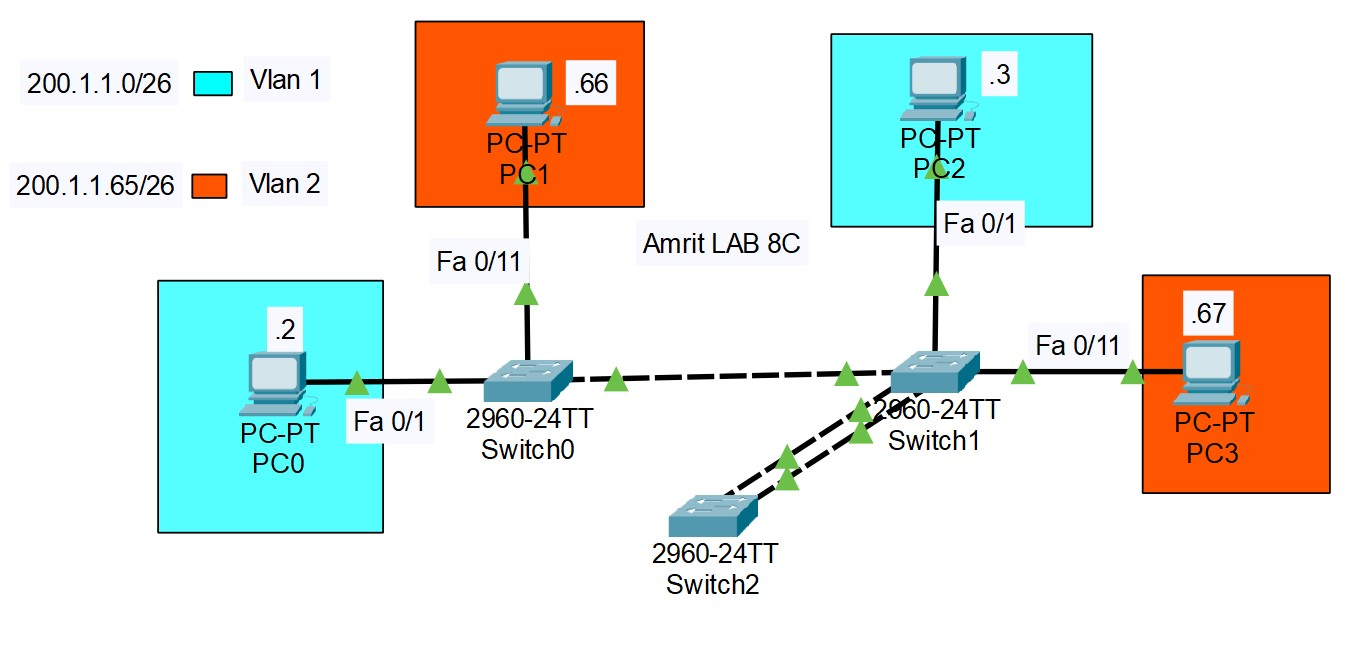
\includegraphics[scale=0.64,cframe=blue 0.5pt 3pt,width=\linewidth]{./FIG/Lab8C.jpg}
    \caption{Network topology Lab 8C}
\end{figure}


\begin{enumerate}

    %%%%%%%%%%%%%%%%%%%%%CCCCCCCCCCCCCCCCCCCCC1111111111111111111111111111111111
    \item\textbf{  Test the connectivity from each computer to another computer. Does ping succeed in all
              cases? State reason}

          %%%%%%%%%%%%%%%%%%%%Copied from A.8 dont make changes, if needed create new

          \addtocontents{lol}{\protect\subsubsection*{C 1 : Testing connectivity  after changing subnet mask to 255.255.255.192}}

          \CMD{./CODES/APE0-1.txt}{Ping from PC0 to PC1}

          \CMD{./CODES/APE0-2.txt}{Ping from PC0 to PC2}

          \CMD{./CODES/APE0-3.txt}{Ping from PC0 to PC3}

          \CMD{./CODES/APE1-2.txt}{Ping from PC1 to PC2}

          \CMD{./CODES/APE1-3.txt}{Ping from PC1 to PC3}

          \CMD{./CODES/APE2-3.txt}{Ping from PC2 to PC3}

          Here we created the two subnets each having usable 62  host . So VLAN 1 and VLAN 2 falls under different subnet and switch is incapable to forward packets between different network. Hence Ping between PCs of same VLAN only succeed.

          %%%%%%%%%%%%%%%%%%%%%%CCCCCCCCCCCCCCCCCCCCC222222222222222222222222222222222
    \item\textbf{ Now the different computers became on different networks, so routing is necessary to
              forward packets between networks. For this set default gateway of PC0 and PC2 as
              200.1.1.1. Similarly the default gateway of PC1 and PC3 as 200.1.1.65.}

          \begin{figure}[H]
              \centering
              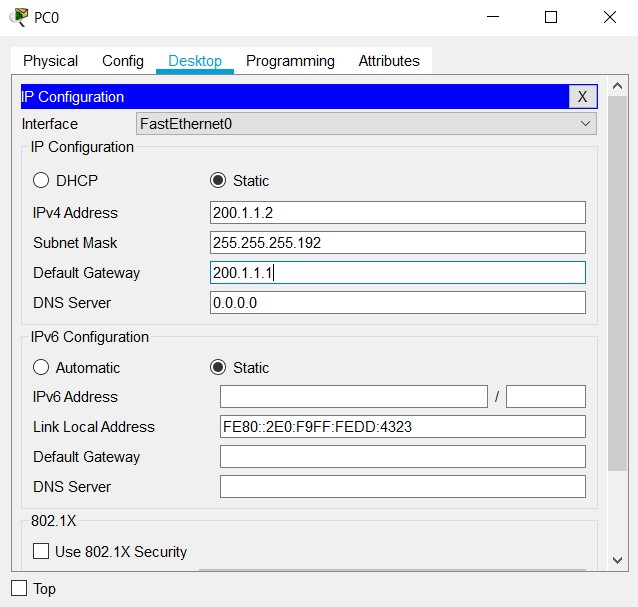
\includegraphics[scale=0.82,cframe=blue 0.5pt 3pt]{./FIG/C_DP0.jpg}
              \caption{Changing Changing Default gateway of PC0 to 200.1.1.1 }
          \end{figure}

          \begin{figure}[H]
              \centering
              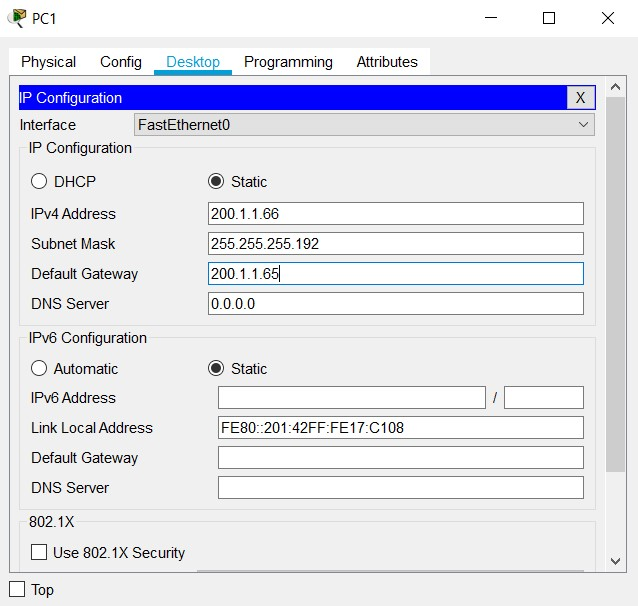
\includegraphics[scale=0.82,cframe=blue 0.5pt 3pt]{./FIG/C_DP1.jpg}
              \caption{Changing Changing Default gateway of PC0 to 200.1.1.65 }
          \end{figure}

          %%%%%%%%%%%%%%%%%%%%%%CCCCCCCCCCCCCCCCCCCCC333333333333333333333333333
    \item\textbf{  Replace Switch2 with a router as Router0 as shown in Figure2 below.}



          %%%%%%%%%%%%%%%%%%%%%CCCCCCCCCCCCCCCCCCCCC44444444444444444444444444444444
    \item\textbf{  Connect interface FastEthernet0/8 of Switch1 to GigabitEthernet0/0 of Router0 having
              IP Address of 200.1.1.1/26, similarly connect interface FastEthernet0/14 of Switch1 to
              GigabitEthernet0/1 of Router0 having IP Address of 200.1.1.65/26}

          \begin{figure}[H]
              \centering
              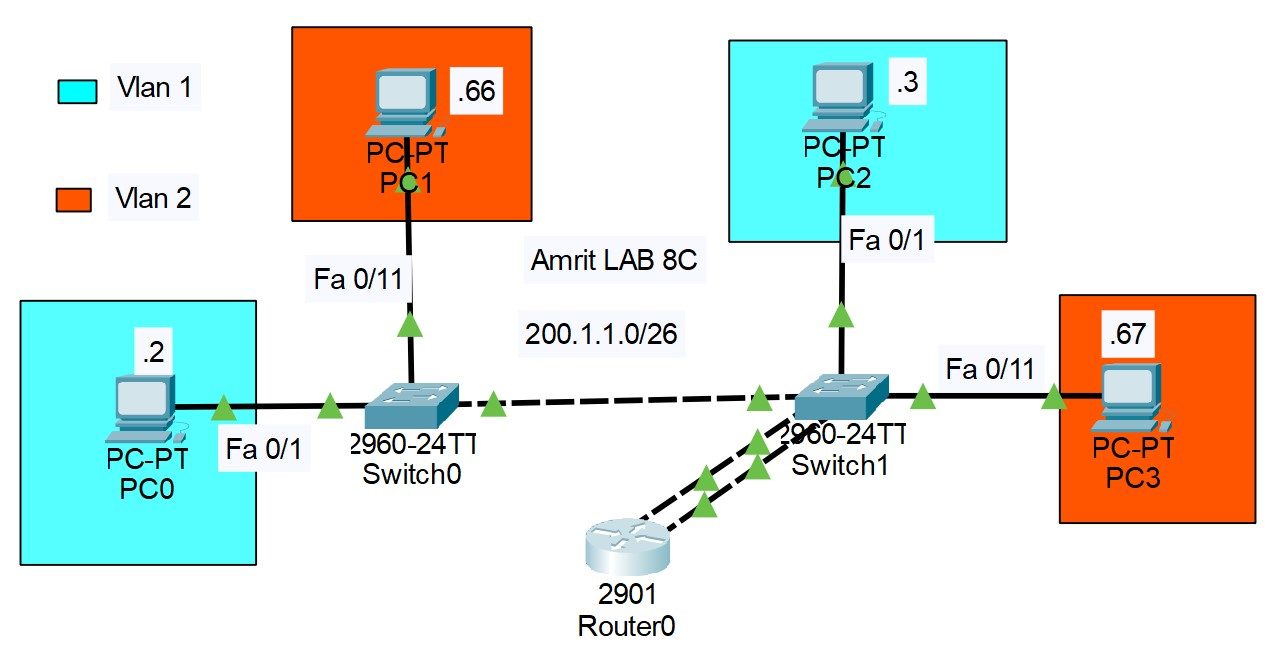
\includegraphics[scale=0.68,cframe=blue 0.5pt 3pt]{./FIG/Lab8C4.jpg}
              \caption{Replacing Switch with Router in Lab 8C}
          \end{figure}

          \CMD{./CODES/C_IP0.txt}{Assigning IP to interface 0/0 in Router 0}

          \CMD{./CODES/C_IP1.txt}{Assigning IP to interface 0/1 in Router 0}


          %%%%%%%%%%%%%%%%%%%%%%CCCCCCCCCCCCCCCCCCCCC55555555555555555555555555555555
    \item\textbf{  Again test the connectivity from each computer to another computer. Does ping succeed
              in all cases? State reason}

          \addtocontents{lol}{\protect\subsubsection*{C.5 : Testing connectivity  after connecting Router 0}}


          %%%%%%%%%%%%%%% Don't edit this .. copied from B.6


          \CMD{./CODES/BPS0-1.txt}{Ping from PC0 to PC1}

          \CMD{./CODES/BPS0-2.txt}{Ping from PC0 to PC2}

          \CMD{./CODES/BPS0-3.txt}{Ping from PC0 to PC3}

          \CMD{./CODES/BPS1-2.txt}{Ping from PC1 to PC2}

          \CMD{./CODES/BPS1-3.txt}{Ping from PC1 to PC3}

          \CMD{./CODES/BPS2-3.txt}{Ping from PC2 to PC3}

          Ping between and among all PCs is successful because Router is introduced and Configured  both interface 0/0 and 0/1  to forward packets between two VLAN1 and VLAN 2 belonging to different subnet.

\end{enumerate}


\pagebreak

%%%%%%%%%%%%%%%%%%%%%%%%%%%%%%%%%%%%%%%%%%%%%%%%%%%%%%%%%%%%%%%%

%
%
%
%

%%%%%%%%%%%%%%%%%%%%%DDDDDDDDDDDDDDDDDDDD
%%%%%%%%%%%%%%%%%%%%%DDDDDDDDDDDDDDDDDDDD
%%%%%%%%%%%%%%%%%%%%%DDDDDDDDDDDDDDDDDDDD
%%%%%%%%%%%%%%%%%%%%%DDDDDDDDDDDDDDDDDDDD
%%%%%%%%%%%%%%%%%%%%%DDDDDDDDDDDDDDDDDDDD
%
%
%
%
%
%
%

\addtocontents{lol}{\protect\subsection*{\HRule \\ Activities D\\ \HRule}}

\addtocontents{lof}{\protect\subsection*{\HRule \\ Activities D\\ \HRule}}

\subsubsection{Activities D}

{\bfseries \textit{D. There are still more than one connections from switch to router. Remove all links between
        Switch1 and Router0. Also reset the IP addresses of all interfaces of router and perform the
        followings:}}


\begin{figure}[H]
    \centering
    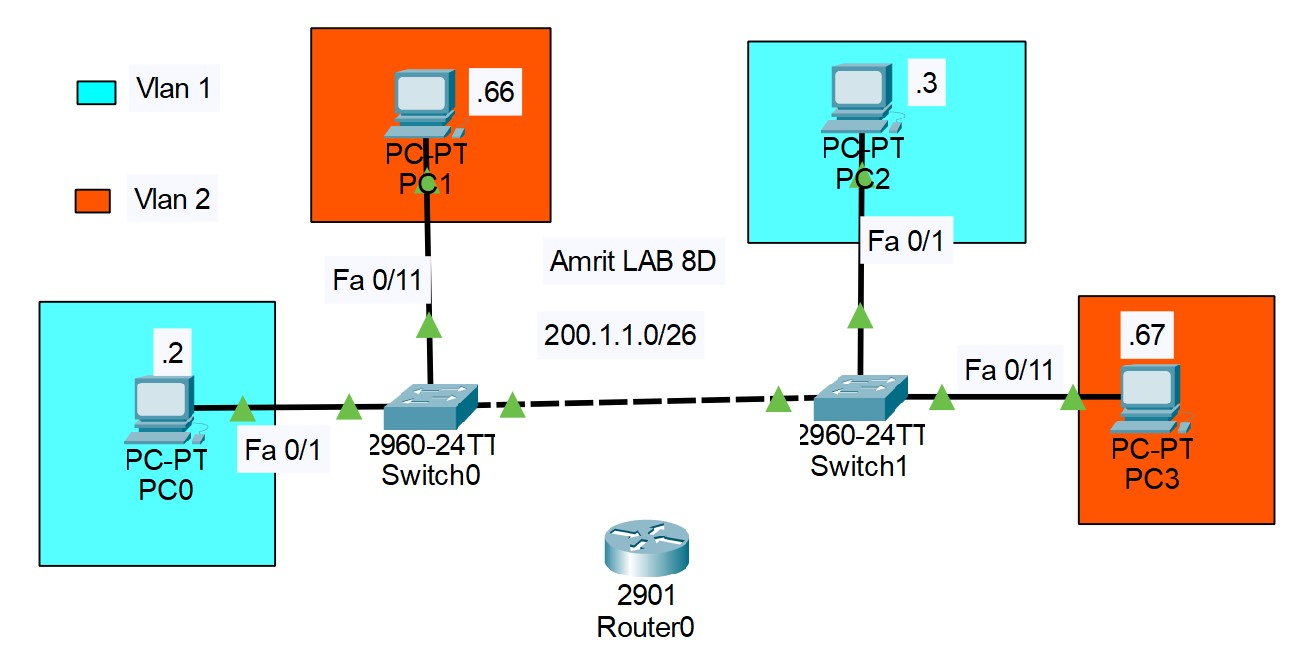
\includegraphics[scale=0.8,cframe=blue 0.5pt 3pt,width=\linewidth]{./FIG/Lab8D.jpg}
    \caption{Network topology Lab 8D after removing all connection}
\end{figure}

\CMD{./CODES/D_RR0.txt}{Resetting all interface in Router 0}



\begin{enumerate}
    %%%%%%%%%%%%%%%%%%%%%DDDDDDDDDDDDDDDDDDDD111111111111111111111111
    %
    \item\textbf{ Configure interfaces FastEthernet0/21 of Switch1 as Trunk port and establish connection
              to the GigabitEthernet0/0 interface of Router0}


          \CMD{./CODES/D_TS1.txt}{Configuring Trunk port to Fa 0/21}

          \begin{figure}[H]
              \centering
              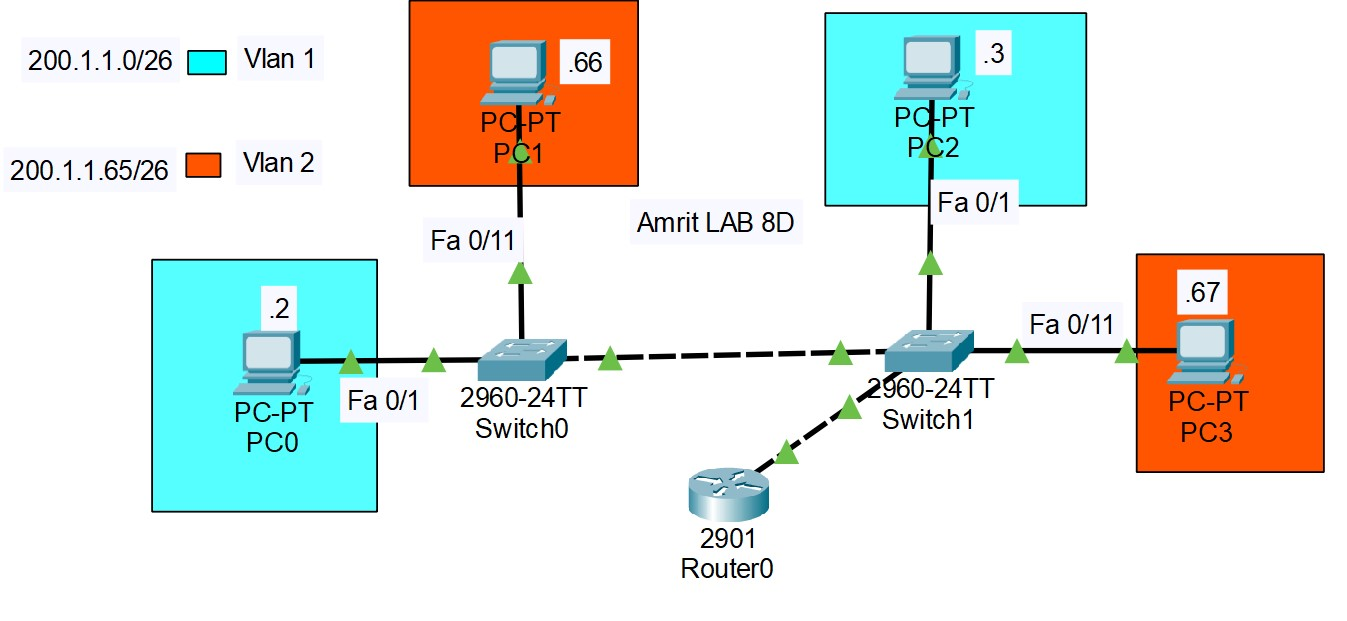
\includegraphics[scale=0.64,cframe=blue 0.5pt 3pt]{./FIG/Lab8D1.jpg}
              \caption{Network topology Lab 8D Connection after Trunk configuraton}
          \end{figure}

          %%%%%%%%%%%%%%%%%%%%%DDDDDDDDDDDDDDDDDDDD2222222222222222222222222
          %
    \item\textbf{ Now configure sub-interfaces as:}
          \begin{verbatim}
           Router0>
          Router0>enable
          Router0#
          Router0\#config t
          Router0(config)#
          Router0(config)#interface gigabitethernet 0/0.1
          Router0(config-subif)#
          Router0(config-subif)#encapsulation dot1Q [VLAN ID i.e. 1 or 2]
          Router0(config-subif)#
          Router0(config-subif)#ip address 200.1.1.1 255.255.255.192
        \end{verbatim}
          \textbf{Similarly configure another sub-interface as GigabitEthernet0/0.2 on same physical
              interface for another VLAN with IP address of 200.1.1.65/26. And finally activate
              this physical interface by using no shutdown command.}

          \CMD{./CODES/D_sub.txt}{Configuring Sub-interfaces 0/0.1 and 0/0.2 and activate}



          %%%%%%%%%%%%%%%%%%%%%DDDDDDDDDDDDDDDDDDDD3333333333333333333333333333333
          %
    \item\textbf{ Again test the connectivity from each computer to another computer. Does ping succeed
              in all cases? State reason}

          \addtocontents{lol}{\protect\subsubsection*{D.3 : Testing connectivity  after connecting Router 0 with sub interfaces}}


          %%%%%%%%%%%%%%% Dont edit this .. copied from B.6


          \CMD{./CODES/BPS0-1.txt}{Ping from PC0 to PC1}

          \CMD{./CODES/BPS0-2.txt}{Ping from PC0 to PC2}

          \CMD{./CODES/BPS0-3.txt}{Ping from PC0 to PC3}

          \CMD{./CODES/BPS1-2.txt}{Ping from PC1 to PC2}

          \CMD{./CODES/BPS1-3.txt}{Ping from PC1 to PC3}

          \CMD{./CODES/BPS2-3.txt}{Ping from PC2 to PC3}


          Here we configured Fa 0/21 of switch 1 in Trunk mode and configured the interface 0/0 of router as sub interfaces 0/0.1 and 0/0.2  having IP belonging to VLAN 1 and VLAN 2 respectively and different subnet too. Here Router forwards packets between those sub interfaces.

          %%%%%%%%%%%%%%%%%%%%%DDDDDDDDDDDDDDDDDDDD4444444444444444444444444
          %
    \item\textbf{ Compare this configuration with previous (i.e. in question no 3).}

          The only physical difference with activity C is it has single interface consisting sub interface in trunk mode between switch 1 and Router 0.


\end{enumerate}





%%%%%%%%%%%%%%%%%%%%%%%%%%%%%%%%%%%%%%%%%%%%%%%%%%%%%%%%%%%%%%%%%%%




\pagebreak

\section{Conclusion}

In this Lab we familiarize ourselves with VLAN , its uses and importance. We also learned to communicate between VLANs on same and different subnets.



\end{document}